\documentclass[12pt,a4paper]{report}

%------------------------------------------------
% Packages
%------------------------------------------------

\usepackage[a4paper,
top=1in,
bottom=1in,
left=1in,
right=1in]{geometry}
\usepackage{fancyhdr}
\usepackage{graphicx}
\usepackage{amsmath}
\usepackage{booktabs}
\usepackage{longtable}
\usepackage{float}
\usepackage{array}
\usepackage{hyperref}
\usepackage{setspace}
\usepackage{titlesec}
\usepackage{listings}
\usepackage{xcolor}
\usepackage{tikz}
\usepackage{eso-pic}
\usepackage{pdfpages}

\onehalfspacing

\hypersetup{
colorlinks=true,
linkcolor=black,
urlcolor=blue
}

\usepackage{tikz}

\newcommand{\pageborder}{%
  \begin{tikzpicture}[remember picture, overlay]
    \draw[line width=0.8pt]
      ([xshift=1.2cm,yshift=-1.2cm]current page.north west)
      rectangle
      ([xshift=-1.2cm,yshift=1.2cm]current page.south east);
  \end{tikzpicture}%
}

%------------------------------------------------
% Title Formatting
%------------------------------------------------
\pagestyle{plain}

\fancypagestyle{front}{
  \fancyhf{}
  \fancyhead[R]{\thepage}
  \renewcommand{\headrulewidth}{0.6pt}
}

\titleformat{\chapter}[display]
{\normalfont\Huge\bfseries}
{\chaptertitlename\ \thechapter}
{0pt}
{}
[\vspace{0.5ex}\titlerule]

\titlespacing*{\chapter}
{0pt}
{-40pt}
{20pt}

% ==============================================================
% DOCUMENT
% ==============================================================
\begin{document}

\pagestyle{front}
\pagenumbering{roman}
\setcounter{page}{1}

\begin{titlepage}
  \addcontentsline{toc}{chapter}{Title Page}
  \thispagestyle{empty}
  \pageborder

  \begin{center}
    \vspace{0.8cm}

    {\Large \bfseries
      A Probabilistic and Explainable Tool for\\ Context-Aware Multimodal Trip Planning Using Generative AI\\[8pt]
    \par}

    \vspace{0.6cm}
    {\large\bfseries Internship Report}

    \vspace{0.4cm}
    {\normalsize Submitted in partial fulfilment of the requirements of the\par}
    {\normalsize\bfseries GRISHMA Summer Research Programme 2026\par}

    \vspace{0.8cm}
    {\large\bfseries Submitted by\par}
    \vspace{0.6cm}
    
    {\Large\bfseries Nikhil Kumar}\\
    
    {\normalsize GRISHMA-STU-2026-18054}
    
    \vspace{0.6cm}

    {\normalsize\itshape Under the supervision of\par}
    {\large\bfseries Dr.\ Nandan Maiti\par}
    {\normalsize Assistant Professor\par}
    {\normalsize Department of Civil Engineering, IIT Kharagpur\par}
    % \vspace{0.1cm}
    
\includegraphics[width=0.26\textwidth]{iit_kgp.jpg}
    \vspace{0.5cm}
    
    {\normalsize\bfseries Department of Civil Engineering\par}
    {\normalsize\bfseries Indian Institute of Technology Kharagpur\par}
    \vspace{0.5cm}
    {\normalsize May -- July 2026\par}

  \end{center}
\end{titlepage}

\setcounter{page}{2}

\thispagestyle{front}
\vspace*{0.5cm}
\begin{center}
  \textbf{\Large DECLARATION}
  \addcontentsline{toc}{chapter}{Declaration}
\end{center}
\vspace{1cm}

\noindent
I, \textbf{Nikhil Kumar (GRISHMA-STU-2026-18054)}, declare that the internship
report titled \textbf{``A Probabilistic and Explainable Tool for Context-Aware
Multimodal Trip Planning Using Generative AI''} submitted to \textbf{Indian
Institute of Technology Kharagpur} as part of the \textbf{GRISHMA Summer Research
Programme 2026} is based on original work carried out by me under the supervision
of \textbf{Dr.\ Nandan Maiti}, Department of Civil Engineering, IIT Kharagpur.

\vspace{0.5cm}
\noindent
This report has not been submitted elsewhere for any degree, diploma, or
qualification. All external sources used have been duly cited.

\vspace{3.5cm}

\noindent
Kharagpur -- 721302 \hfill \textbf{Nikhil Kumar}\\
July 2026 \hfill GRISHMA-STU-2026-18054

\newpage

\thispagestyle{front}
\vspace*{0.5cm}
\begin{center}
  \textbf{\Large ABSTRACT}
  \addcontentsline{toc}{chapter}{Abstract}
\end{center}
\vspace{1cm}

\noindent
Most navigation systems today update routes only after a disruption has already
been detected by sensors -- they are reactive by design. This project builds an
\textbf{anticipatory} alternative for Kolkata, India.

\vspace{0.5cm}
\noindent
The system, \textbf{traffic-ai}, pulls unstructured text from nine live sources
(news RSS feeds, TomTom traffic incidents, official advisories, weather APIs)
and uses a Large Language Model to extract structured disruption events from that
text \textit{before} a commuter travels. Each event carries a severity score
$\sigma$ and a confidence weight $\kappa$. A Temporal Heterogeneous Graph Neural
Network (HGNN) then adjusts those confidence values using city-wide spatial
context. A Bayesian fusion layer converts the signals into per-road disruption
probabilities, which are used to colour-code and rank candidate routes on a
Leaflet.js map.

\vspace{0.5cm}
\noindent
The system supports eight transport modes spanning drive, walk, bike, all five
Kolkata Metro lines, and bus. The API is split into two steps: routes appear on
screen within $\sim$2~s while the slower LLM pipeline ($\sim$30--60~s) fills in
risk scores in the background.

\vspace{0.5cm}

\begin{table}[H]
\centering
\begin{tabular}{ll}
\toprule
\textbf{Aspect} & \textbf{Summary} \\
\midrule
Pilot city          & Kolkata, India \\
Data sources        & 9 (structured + unstructured) \\
Transport modes     & 8 \\
LLM backend         & OpenRouter / Gemini / Ollama (configurable) \\
Graph model         & Temporal HAN -- 3 output heads \\
Probabilistic layer & Bayesian fusion with time-of-day priors \\
\bottomrule
\end{tabular}
\end{table}

\newpage


\vspace{-50pt}
\tableofcontents
\newpage
\listoffigures
\newpage
\listoftables
\newpage

\pagenumbering{arabic}
% \pagestyle{main}

\chapter{Introduction}

\section{Context}

Kolkata's road network carries millions of trips daily across a mix of private
vehicles, metros, busses, and pedestrians. Disruptions -- waterlogging, VIP
convoys, accidents, road closures -- are frequent and hard to predict from
sensor data alone because a large share of disruption information first appears
in news articles and official advisories, not on roads.

Existing navigation tools (Google Maps, Apple Maps) react to congestion after
it shows up in GPS probe data, often minutes to hours after the event begins.
This project asks whether reading that unstructured text \textit{before travel}
can produce better route recommendations.

\section{Problem Statement}

\begin{table}[H]
\centering

\begin{tabular}{lll}
\toprule
\textbf{Dimension} & \textbf{Current systems} & \textbf{This project} \\
\midrule
Data types used     & Structured only          & Structured + unstructured \\
Timing              & After disruption         & Before disruption \\
Objective           & Minimise travel time     & Minimise risk-adjusted time \\
Uncertainty         & Deterministic            & Probabilistic \\
Explainability      & None                     & HGNN attention weights \\
Multimodal          & Limited                  & 8 modes inc.\ metro and bus \\
\bottomrule
\end{tabular}
\caption{Reactive vs.\ anticipatory trip planning}
\end{table}

\section{Research Hypotheses}

\begin{table}[H]
\centering

\begin{tabular}{cp{11.5cm}}
\toprule
\textbf{ID} & \textbf{Hypothesis} \\
\midrule
H1 & LLM-derived contextual signals improve disruption detection accuracy
     over structured-data-only baselines. \\
H2 & Probabilistic, risk-aware routing improves travel-time reliability
     under uncertain conditions. \\
H3 & Exposing HGNN attention weights as route explanations increases
     commuter trust in system recommendations. \\
\bottomrule
\end{tabular}
\caption{Guiding hypotheses}
\end{table}

\section{Scope of Internship}

\begin{table}[H]
\centering
\caption{Work carried out during the internship}
\begin{tabular}{clc}
\toprule
\textbf{\#} & \textbf{Contribution} & \textbf{Status} \\
\midrule
1  & LLM disruption extraction pipeline (Layer 1)               & Done \\
2  & Multi-factor confidence scoring + impact duration           & Done \\
3  & Temporal HGNN -- training loop + inference                 & Done \\
4  & Bayesian probabilistic fusion (Layer 2)                     & Done \\
5  & Weather Severity Index per route                            & Done \\
6  & Kolkata Metro integration (5 lines, timetable, next-train)  & Done \\
7  & Bus transit graph + BFS routing engine                      & Done \\
8  & Multimodal routing orchestration                            & Done \\
9  & FastAPI backend (11 endpoints)                              & Done \\
10 & Leaflet.js frontend + map overlays                          & Done \\
11 & CVaR risk-aware routing (Layer 3)                           & In progress \\
\bottomrule
\end{tabular}
\end{table}

\section{Report Structure}

\begin{table}[H]
\centering
\begin{tabular}{cl}
\toprule
\textbf{Chapter} & \textbf{Content} \\
\midrule
2 & System architecture, data sources, API design \\
3 & Implementation -- Layers 1, 2, routing, database \\
4 & Results, UI screenshots, performance metrics \\
5 & Conclusion and future work \\
\bottomrule
\end{tabular}
\end{table}

\chapter{System Architecture and Problem Formulation}

% ==============================================================
\section{Notation}
% ==============================================================

\begin{table}[H]
\centering
\caption{Mathematical notation used throughout the report}
\begin{tabular}{p{2.8cm} p{10cm}}
\toprule
\textbf{Symbol} & \textbf{Definition} \\
\midrule
$\mathcal{G} = (V, E)$
  & Directed road graph; $V$ = intersections, $E$ = road segments \\
$e \in E$
  & A directed road edge (segment) \\
$\mathcal{A} = \{a_1, \dots, a_N\}$
  & Set of $N$ ingested articles / traffic incidents \\
$\mathcal{D} = \{d_1, \dots, d_M\}$
  & Set of $M$ extracted disruption events after LLM processing \\
$\sigma_i \in \{2, 5, 10\}$
  & Severity score of event $d_i$: low $= 2$, medium $= 5$, high $= 10$ \\
$\kappa_i \in [0, 1]$
  & Confidence weight of event $d_i$ \\
$\hat{\kappa}_i$
  & HGNN-adjusted confidence for event $d_i$ \\
$\kappa_i^{\text{final}}$
  & Blended confidence after HGNN correction \\
$Z_e(t) \in \{0, 1\}$
  & Binary disruption state of edge $e$ at time $t$ \\
$\pi_e^{\text{prior}}(t)$
  & Time-of-day prior disruption probability for edge $e$ \\
$\pi_e^{\text{post}}(t)$
  & Posterior disruption probability after Bayesian update \\
$\pi_e^{\text{final}}(t)$
  & Final per-edge probability after HGNN blend \\
$\mathcal{R} = \{r_1, \dots, r_K\}$
  & Set of $K$ candidate routes computed for a query \\
$\rho(r)$
  & Aggregate risk score of route $r$ \\
$t_r$
  & Expected travel time of route $r$ \\
$\mathcal{C}(r)$
  & Composite route cost used for ranking \\
$d_m, r_m$
  & Duration multiplier and recency multiplier \\
$\mathbf{h}_v^{(\phi)}$
  & Hidden embedding of node $v$ of type $\phi$ in the HGNN \\
$\alpha_{uv}$
  & Attention coefficient between nodes $u$ and $v$ \\
$\beta_\psi$
  & Semantic attention weight for meta-path $\psi$ \\
\bottomrule
\end{tabular}
\end{table}

% ==============================================================
\section{Formal Problem Definition}
% ==============================================================

Let $\mathcal{G} = (V, E)$ be the directed road graph of Kolkata.
Each edge $e \in E$ carries a free-flow travel time $t_e^0$ and a
disruption state $Z_e(t) \in \{0, 1\}$, which is latent and
must be inferred from external signals.

\medskip
\noindent
A user query $q = (\text{origin}, \text{destination}, \text{mode}, t)$
arrives at time $t$. The system must return a ranked list of routes
$r_1 \prec r_2 \prec \cdots \prec r_K$ from origin to destination
under mode constraints, where the ranking criterion is a composite
cost that accounts for both expected travel time and disruption risk.

\medskip
\noindent
The key challenge is that $Z_e(t)$ is not directly observable.
It must be estimated from unstructured signals — news articles,
RSS feeds, official advisories — that carry noisy, partial, and
sometimes conflicting information about road conditions.

\medskip
\noindent
\textbf{Objective.} Find the route $r^*$ that minimises the
risk-adjusted composite cost:
\begin{equation}
  r^* \;=\; \arg\min_{r \in \mathcal{R}}\; \mathcal{C}(r)
  \;=\; \arg\min_{r \in \mathcal{R}}\;
        t_r \cdot \Bigl(1 + \frac{\rho(r)}{10}\Bigr)
  \label{eq:objective}
\end{equation}

where $\rho(r)$ is the aggregate risk score of route $r$, derived from
the posterior edge disruption probabilities $\pi_e^{\text{final}}(t)$
computed through the three-layer pipeline described below.

% ==============================================================
\section{Layer Overview}
% ==============================================================

The system processes each query through three sequential layers.

\begin{table}[H]
\centering
\caption{System layer summary}
\begin{tabular}{clp{5cm}c}
\toprule
\textbf{Layer} & \textbf{Function} & \textbf{Key output} & \textbf{Status} \\
\midrule
1 & LLM extraction + HGNN refinement
  & $(\sigma_i, \kappa_i^{\text{final}})$ per event $d_i$
  & Complete \\
2 & Bayesian probabilistic fusion
  & $\pi_e^{\text{final}}(t)$ per edge $e$
  & Complete \\
3 & CVaR risk-aware routing
  & ranked routes $r_1 \prec \cdots \prec r_K$
  & In progress \\
\bottomrule
\end{tabular}
\end{table}

\noindent
The end-to-end pipeline for a single user query is:

\begin{equation}
  \mathcal{A}
  \;\xrightarrow{\text{pre-filter}}\;
  \tilde{\mathcal{A}}
  \;\xrightarrow{\text{LLM}}\;
  \mathcal{D}
  \;\xrightarrow{\text{HGNN}}\;
  \{\kappa_i^{\text{final}}\}
  \;\xrightarrow{\text{Bayes}}\;
  \{\pi_e^{\text{final}}\}
  \;\xrightarrow{\text{score}}\;
  \{\rho(r)\}
  \;\xrightarrow{\text{rank}}\;
  r^*
  \label{eq:pipeline}
\end{equation}

% ==============================================================
\section{Data Ingestion Sources}
% ==============================================================

\begin{longtable}{p{4.0cm} p{2.6cm} p{6.4cm}}
\toprule
\textbf{Source} & \textbf{Type} & \textbf{What it provides} \\
\midrule
\endhead
TomTom Incidents API v5~\cite{tomtom2024}
  & Structured, live
  & Accidents, closures, road-works with GPS coordinates;
    2{,}500 free req/day \\[4pt]
Google News RSS \texttt{when:2d}
  & Unstructured
  & City-wide Kolkata disruption news scoped to last 2 days \\[4pt]
NewsAPI
  & Unstructured
  & Per-road keyword search, last 24 h \\[4pt]
OpenWeatherMap~\cite{openweathermap2024}
  & Structured, live
  & Precipitation intensity, wind speed, visibility \\[4pt]
Kolkata Police (via RSS)
  & Unstructured
  & Official traffic advisories \\[4pt]
KMRC~\cite{kmrc2024}
  & Unstructured
  & Metro service disruption notices \\[4pt]
WB Disaster Management
  & Unstructured
  & Flood and cyclone alerts \\[4pt]
Indian Railways (erail.in)
  & Structured
  & Delayed trains at Howrah / Sealdah \\[4pt]
KMC Waterlogging (RSS)
  & Unstructured
  & Waterlogging hotspot reports \\
\bottomrule
\end{longtable}

% ==============================================================
\section{Two-Step API Design}
% ==============================================================

Equation~\eqref{eq:pipeline} has two distinct latency regimes.
Route geometry computation on the cached OSM graph takes
$\sim$2~s; the LLM pipeline over all articles takes 30--60~s.
Blocking the user interface on the slower step is unacceptable,
so the pipeline is split at the HGNN boundary:

\begin{table}[H]
\centering
\caption{Two-step decoupled request flow}
\begin{tabular}{p{0.46\textwidth} p{0.46\textwidth}}
\toprule
\textbf{Step 1 --- \texttt{POST /api/route} ($\sim$2 s)} &
\textbf{Step 2 --- \texttt{POST /api/disruptions} ($\sim$30--60 s)} \\
\midrule
Computes $\mathcal{R}$ using OSMnx Yen's $k$-shortest paths.
Returns GeoJSON immediately.
All routes assigned placeholder $\rho(r) = 0$, shown green. &
Executes steps $\tilde{\mathcal{A}} \to \mathcal{D} \to \{\kappa_i^{\text{final}}\}
\to \{\pi_e^{\text{final}}\} \to \{\rho(r)\}$.
Map updated with risk colours and disruption markers. \\
\bottomrule
\end{tabular}
\end{table}

% ==============================================================
\section{Transport Modes and Graph Construction}
% ==============================================================

For each transport mode $m$, a separate graph $\mathcal{G}_m = (V_m, E_m)$
is maintained:

\begin{table}[H]
\centering
\caption{Graph structure per transport mode}
\begin{tabular}{l l l}
\toprule
\textbf{Mode} & \textbf{Graph} & \textbf{Edge weight $w_e$} \\
\midrule
\texttt{drive}        & OSMnx drive graph        & Free-flow travel time \\
\texttt{walk}         & OSMnx pedestrian graph   & Walking time at 5 km/h \\
\texttt{bike}         & OSMnx cycling graph      & Cycling time at 15 km/h \\
\texttt{metro}        & 5-line station graph     & Scheduled travel time + headway \\
\texttt{metro+walk}   & Drive + metro + walk     & Composite (access + ride + egress) \\
\texttt{metro+bike}   & Bike + metro + bike      & Composite \\
\texttt{metro+drive}  & Drive + metro + drive    & Composite \\
\texttt{bus}          & Bus stop graph           & Estimated inter-stop time \\
\bottomrule
\end{tabular}
\end{table}

For multimodal journeys the total composite cost is:
\begin{equation}
  t_r^{\text{multimodal}}
  \;=\; t_r^{\text{access}} + t_r^{\text{transit}} + t_r^{\text{egress}}
  \label{eq:multimodal}
\end{equation}

where each leg uses the edge weights appropriate to its mode.

% ==============================================================
\section{Complete API Surface}
% ==============================================================

\begin{table}[H]
\centering
\caption{REST API endpoints --- built with FastAPI~\cite{fastapi2024}}
\begin{tabular}{l l p{7cm}}
\toprule
\textbf{Method} & \textbf{Endpoint} & \textbf{Description} \\
\midrule
GET  & \texttt{/}                            & Leaflet.js~\cite{leaflet2024} map frontend \\
GET  & \texttt{/api/locations}               & Localities, metro stations, bus stops \\
POST & \texttt{/api/route}                   & Step 1 --- compute $\mathcal{R}$ only \\
POST & \texttt{/api/disruptions}             & Step 2 --- full pipeline, returns $\rho(r)$ \\
POST & \texttt{/api/explain-route}           & HGNN attention weights per event \\
GET  & \texttt{/api/metro-overlay}           & GeoJSON of all 5 metro lines \\
GET  & \texttt{/api/metro-lines}             & Timetable summary per line \\
GET  & \texttt{/api/next-metro/\{station\}}  & Next $n$ trains (live IST time) \\
GET  & \texttt{/api/bus-overlay}             & GeoJSON of all bus stops \\
GET  & \texttt{/api/bus-network}             & Full bus route and stop data \\
GET  & \texttt{/api/hgnn-status}             & Model weights loaded / ready flag \\
\bottomrule
\end{tabular}
\end{table}

\chapter{Methodology}

% ==============================================================
\section{Layer 1 --- LLM Disruption Intelligence}
% ==============================================================

\subsection{Article Pre-filter}

Let $\mathcal{A} = \{a_1, \dots, a_N\}$ be the raw article set fetched
from all sources. Before incurring any LLM cost, each article $a_i$ is
evaluated against three binary predicates:

\begin{align}
  f_{\text{age}}(a_i)  &= \mathbf{1}\!\left[\,t_{\text{now}} - t_{a_i} \leq T_{\max}\right],
  \quad T_{\max} = 48\text{ h} \label{eq:filter_age}\\
  f_{\text{geo}}(a_i)  &= \mathbf{1}\!\left[\,\ell_{a_i} \in \mathcal{B}_{\text{KOL}}\right]
  \label{eq:filter_geo}\\
  f_{\text{rel}}(a_i)  &= \mathbf{1}\!\left[\,\exists\, w \in \mathcal{W} : w \in a_i\right]
  \label{eq:filter_rel}
\end{align}

where $\mathcal{B}_{\text{KOL}}$ is the Kolkata bounding box
$(22.45^\circ\text{N},\,88.24^\circ\text{E})$ to
$(22.63^\circ\text{N},\,88.46^\circ\text{E})$,
and $\mathcal{W}$ is a curated keyword vocabulary of transport terms.
Only articles satisfying all three predicates form the filtered set:
\begin{equation}
  \tilde{\mathcal{A}} = \bigl\{\,a_i \in \mathcal{A} \;\mid\;
  f_{\text{age}}(a_i) \wedge f_{\text{geo}}(a_i) \wedge f_{\text{rel}}(a_i)\bigr\}
  \label{eq:filtered_set}
\end{equation}

\subsection{LLM Structured Extraction}

Each article $a_i \in \tilde{\mathcal{A}}$ is passed to a large language
model $\mathcal{M}$ that is constrained to return a structured object
conforming to \texttt{TrafficEventSchema}:
\begin{equation}
  d_i = \mathcal{M}(a_i) =
  \bigl(\text{type}_i,\;\ell_i,\;\sigma_i,\;\kappa_i^{\text{llm}},\;
        \tau_i,\;\delta_i,\;b_i^{\text{future}}\bigr)
  \label{eq:llm_extraction}
\end{equation}

where $\ell_i$ is the extracted location string (mandatory),
$\tau_i$ is the time mentioned, $\delta_i$ is the estimated impact
duration in minutes, and $b_i^{\text{future}} \in \{0,1\}$ flags
planned events. The severity $\sigma_i$ is discretised as:
\begin{equation}
  \sigma_i =
  \begin{cases}
    2  & \text{if severity} = \texttt{low} \\
    5  & \text{if severity} = \texttt{medium} \\
    10 & \text{if severity} = \texttt{high}
  \end{cases}
  \label{eq:severity_map}
\end{equation}

\textbf{Location enforcement.} If $\ell_i = \varnothing$ after the
primary extraction:
\begin{equation}
  d_i =
  \begin{cases}
    \mathcal{M}_{\text{loc}}(a_i) & \text{if } \kappa_i^{\text{llm}} \geq 0.6
      \quad \text{(location-retry pass)} \\
    \text{discard}                & \text{if } \kappa_i^{\text{llm}} < 0.6
  \end{cases}
  \label{eq:location_enforcement}
\end{equation}

where $\mathcal{M}_{\text{loc}}$ is a focused second prompt requesting
only the location field. This prevents null-location events from
inflating route risk scores.

\subsection{Multi-Factor Confidence Scoring}

The raw LLM confidence $\kappa_i^{\text{llm}}$ is adjusted by three
independent reliability factors before being used downstream:
\begin{equation}
  \kappa_i^{\text{rule}} =
  \kappa_i^{\text{llm}}
  \;\cdot\; \lambda_s(s_i)
  \;\cdot\; \lambda_a(t_{\text{now}} - t_{a_i})
  \;\cdot\; \lambda_\ell(\ell_i)
  \label{eq:rule_confidence}
\end{equation}

\begin{table}[H]
\centering
\caption{Confidence adjustment factors in Eq.~\eqref{eq:rule_confidence}}
\begin{tabular}{llp{7.5cm}}
\toprule
\textbf{Factor} & \textbf{Symbol} & \textbf{Definition} \\
\midrule
Source reliability
  & $\lambda_s(s_i) \in [0.6, 1.0]$
  & TomTom = 1.0; official scrapers = 0.9;
    RSS city = 0.75; NewsAPI = 0.7 \\[4pt]
Age decay
  & $\lambda_a(\Delta t) \in [0.5, 1.0]$
  & $\Delta t \leq 1\text{ h}: 1.0$;\;
    $\leq 6\text{ h}: 0.9$;\;
    $\leq 24\text{ h}: 0.75$;\;
    older: $0.5$ \\[4pt]
Location quality
  & $\lambda_\ell(\ell_i) \in [0.7, 1.0]$
  & \texttt{direct}: 1.0;\;
    \texttt{road\_name}: 0.95;\;
    \texttt{landmark}: 0.85;\;
    \texttt{llm\_inferred}: 0.7 \\
\bottomrule
\end{tabular}
\end{table}

\subsection{Event Risk Scoring}

The weighted score for a single event $d_i$ is:
\begin{equation}
  w_i = \sigma_i \;\cdot\; \kappa_i^{\text{final}}
        \;\cdot\; d_m(\delta_i) \;\cdot\; r_m(\Delta t_i)
  \label{eq:weighted_score}
\end{equation}

The duration multiplier $d_m$ penalises long-lasting disruptions:
\begin{equation}
  d_m(\delta_i) =
  \begin{cases}
    2.0 & \delta_i \geq 1440 \text{ min} \quad (\geq\!1\text{ day})\\
    1.5 & 480 \leq \delta_i < 1440 \quad (\geq\!8\text{ h})\\
    1.2 & 120 \leq \delta_i < 480  \quad (\geq\!2\text{ h})\\
    1.0 & \text{otherwise}
  \end{cases}
  \label{eq:duration_mult}
\end{equation}

The recency multiplier $r_m$ down-weights stale events:
\begin{equation}
  r_m(\Delta t_i) =
  \begin{cases}
    1.00 & \Delta t_i \leq 1\text{ h} \\
    0.90 & 1 < \Delta t_i \leq 6\text{ h} \\
    0.75 & 6 < \Delta t_i \leq 24\text{ h} \\
    0.50 & \Delta t_i > 24\text{ h}
  \end{cases}
  \label{eq:recency_mult}
\end{equation}

The aggregate risk score for route $r$ is the sum over all events
that (i) are matched spatially to the route corridor, (ii) are
currently active ($b_i^{\text{future}} = 0$), and (iii) are recent:
\begin{equation}
  \rho(r) = \sum_{\substack{d_i \in \mathcal{D}_r \\ b_i^{\text{future}}=0}}
            w_i
  \label{eq:route_risk}
\end{equation}

where $\mathcal{D}_r \subseteq \mathcal{D}$ is the set of events
matched to route $r$. Risk levels are thresholded as:
\begin{equation}
  \text{level}(r) =
  \begin{cases}
    \textsc{Critical} & \rho(r) \geq 25 \\
    \textsc{High}     & 12 \leq \rho(r) < 25 \\
    \textsc{Moderate} & 5  \leq \rho(r) < 12 \\
    \textsc{Low}      & 0  < \rho(r) < 5 \\
    \textsc{Clear}    & \rho(r) = 0
  \end{cases}
  \label{eq:risk_levels}
\end{equation}

\chapter{Results and System Demonstration}

\section{Performance Metrics}

\begin{table}[H]
\centering
\resizebox{0.7\textwidth}{!}{
\begin{tabular}{ll}
\toprule
\textbf{Metric} & \textbf{Observed value} \\
\midrule
Route computation (\texttt{/api/route})             & $\sim$ 2 s \\
LLM pipeline (\texttt{/api/disruptions})            & 30 -- 60 s \\
OSM graph load from pickle cache                    & $\sim$ 2 s \\
OSM graph first-time download                       & $\sim$ 30 -- 60 s (once) \\
Data sources integrated                             & 9 \\
Transport modes supported                           & 8 \\
Pre-defined Kolkata localities                      & 15 + metro stations + bus stops \\
Metro lines                                         & 5 \\
Event types extractable                             & 13 \\
HGNN output heads                                   & 3 \\
TomTom free-tier capacity                           & 2{,}500 req/day \\
LLM rate-limit handling                             & Exponential backoff on 429 \\
\bottomrule
\end{tabular}
}
\caption{System performance summary}
\end{table}

% -------------------------------------------------------------------
\section{UI Screenshots}
% -------------------------------------------------------------------

\noindent
\textit{Instructions for compilation: place your \texttt{.png} screenshots
in the same folder as the \texttt{.tex} files and uncomment the relevant
\texttt{\textbackslash includegraphics} line inside each figure environment.}

\bigskip

% -------  Figure 4.1  -------
\begin{figure}[H]
\centering
% Uncomment the line below and replace filename when screenshot is ready:
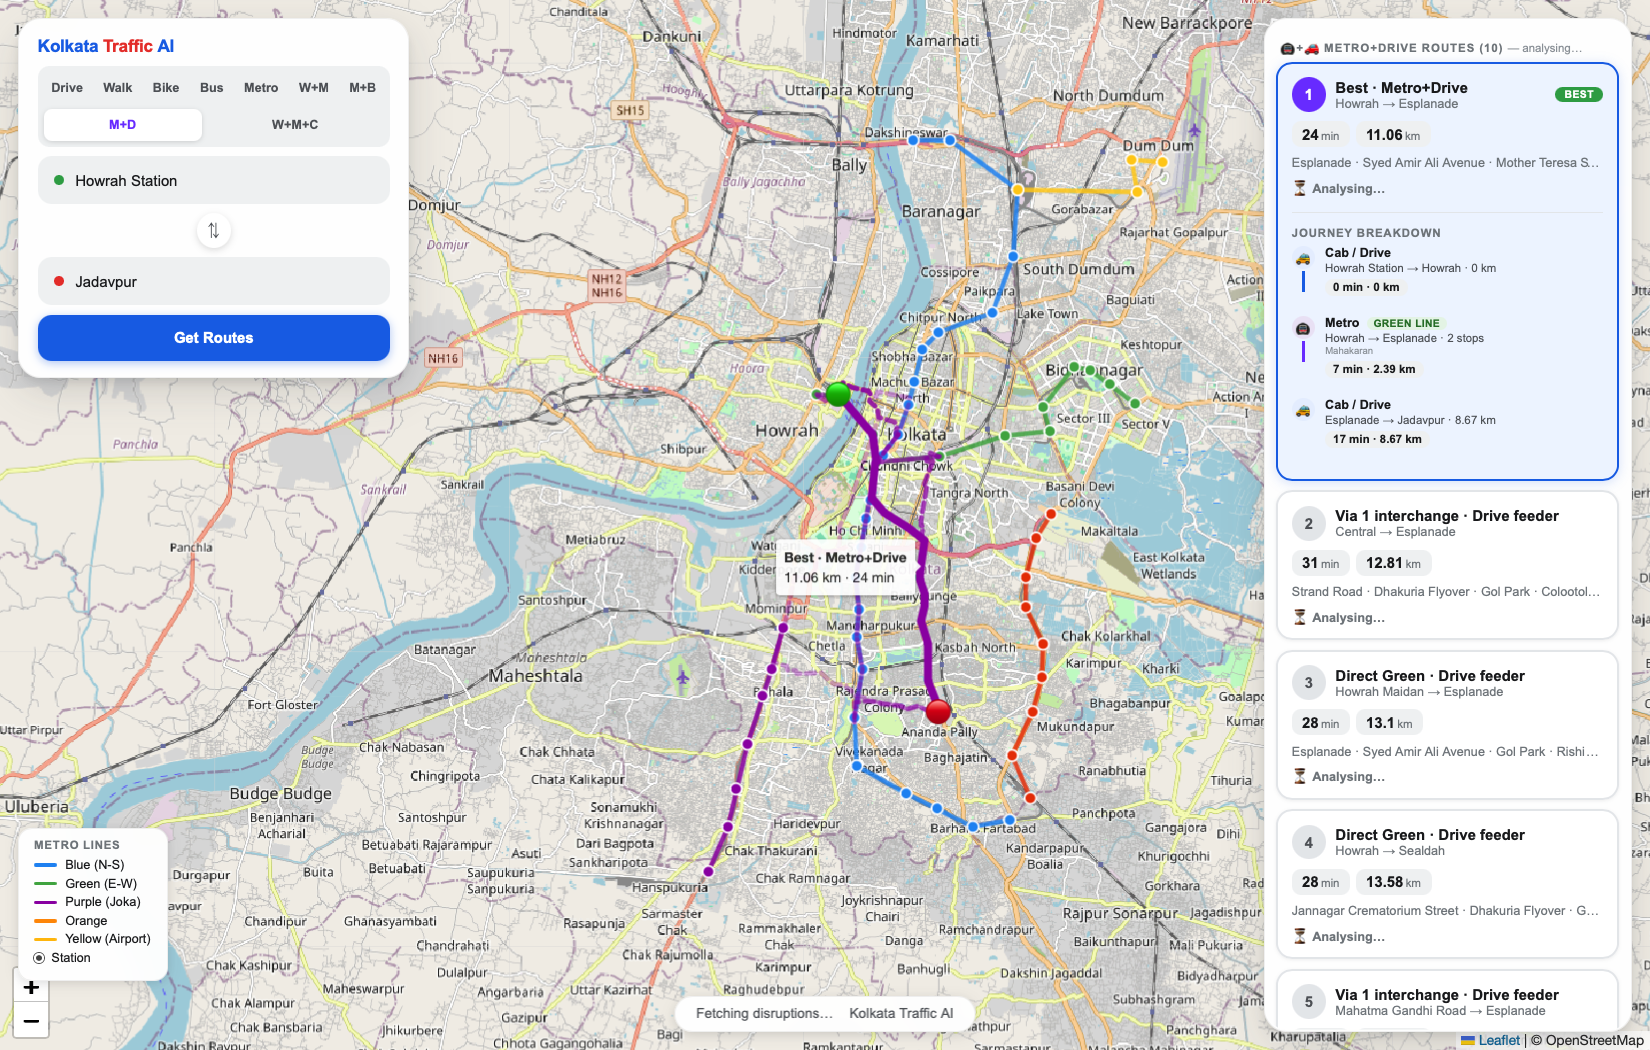
\includegraphics[width=0.8\linewidth]{ui1.png}
\caption{Step~1 --- routes rendered before disruption analysis.}
\label{fig:step1}
\end{figure}

% -------  Figure 4.2  -------
\begin{figure}[H]
\centering
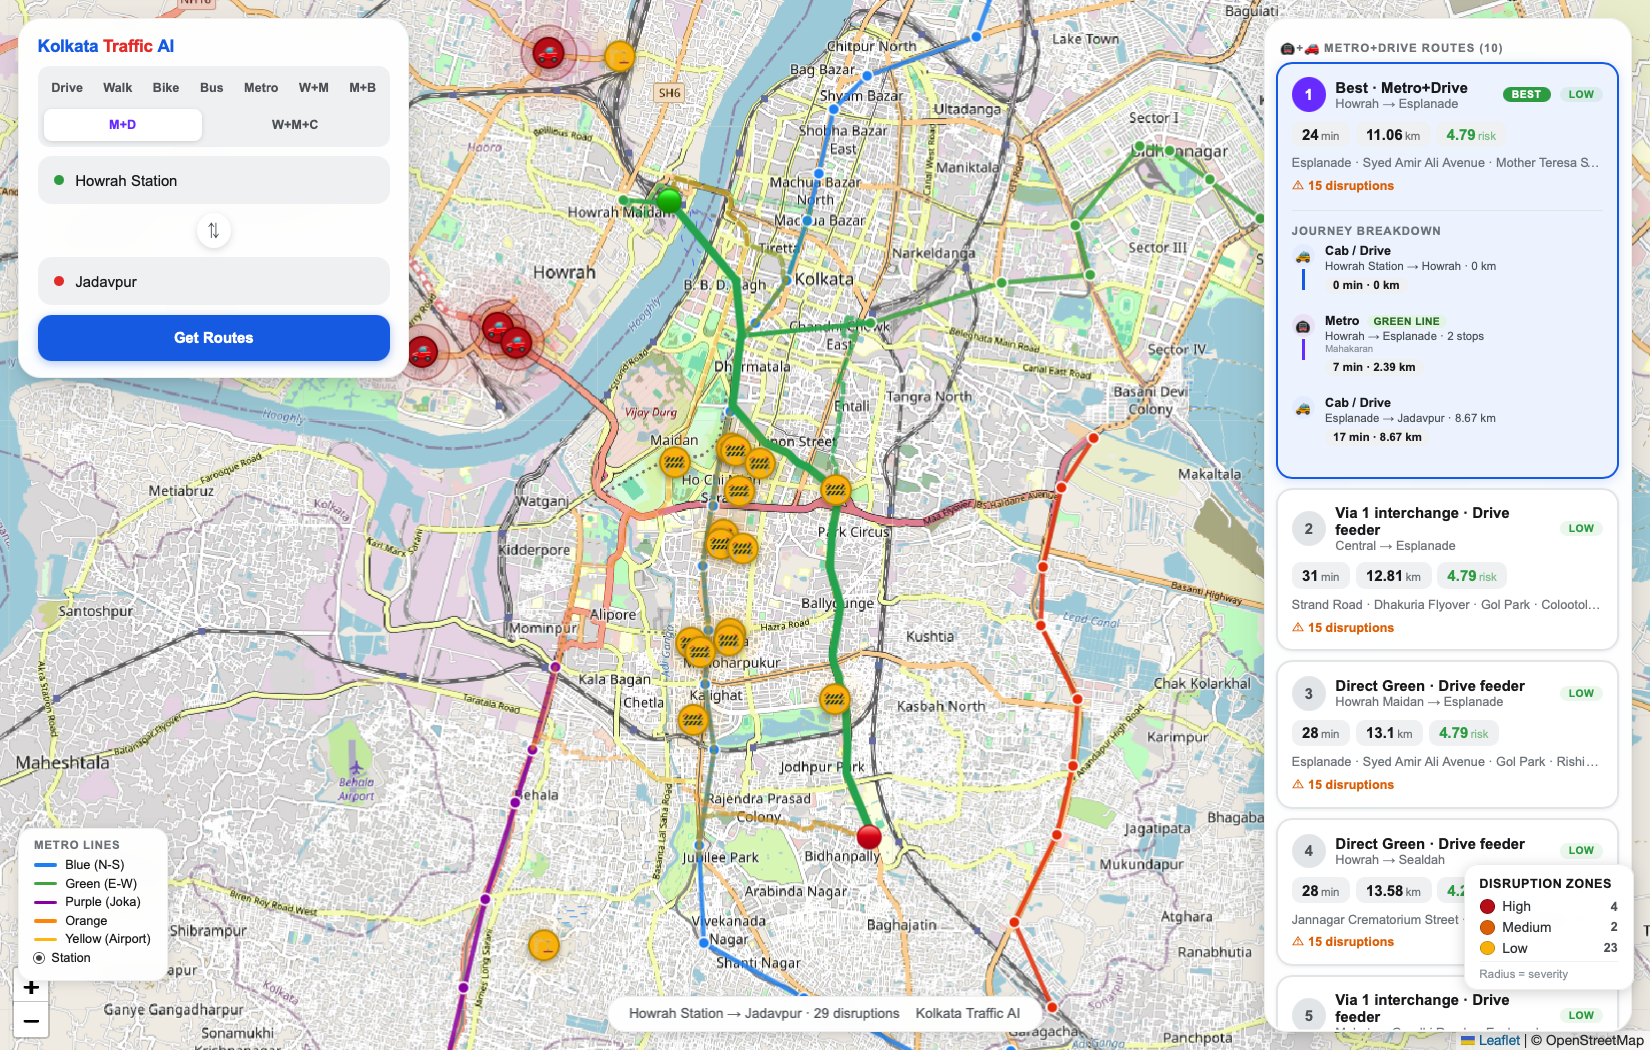
\includegraphics[width=1\linewidth]{ui2.png}
\caption{Step~2 --- routes coloured by risk; disruption panel populated.}
\label{fig:step2}
\end{figure}

% -------  Figure 4.3  -------
\begin{figure}[H]
\centering
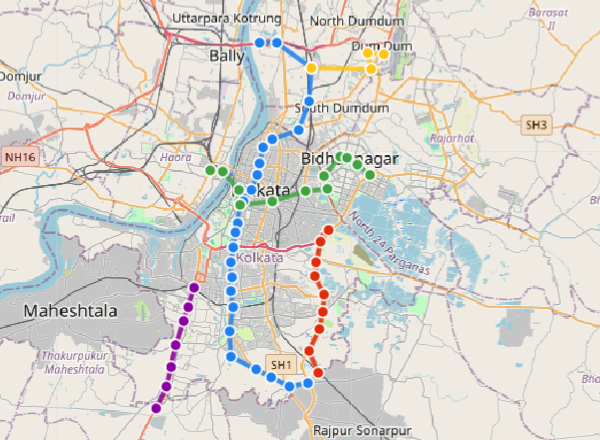
\includegraphics[width=1\linewidth]{ui_metro.png}
\caption{Metro overlay.}
\label{fig:metro}
\end{figure}

% -------  Figure 4.4  -------
\begin{figure}[H]
\centering
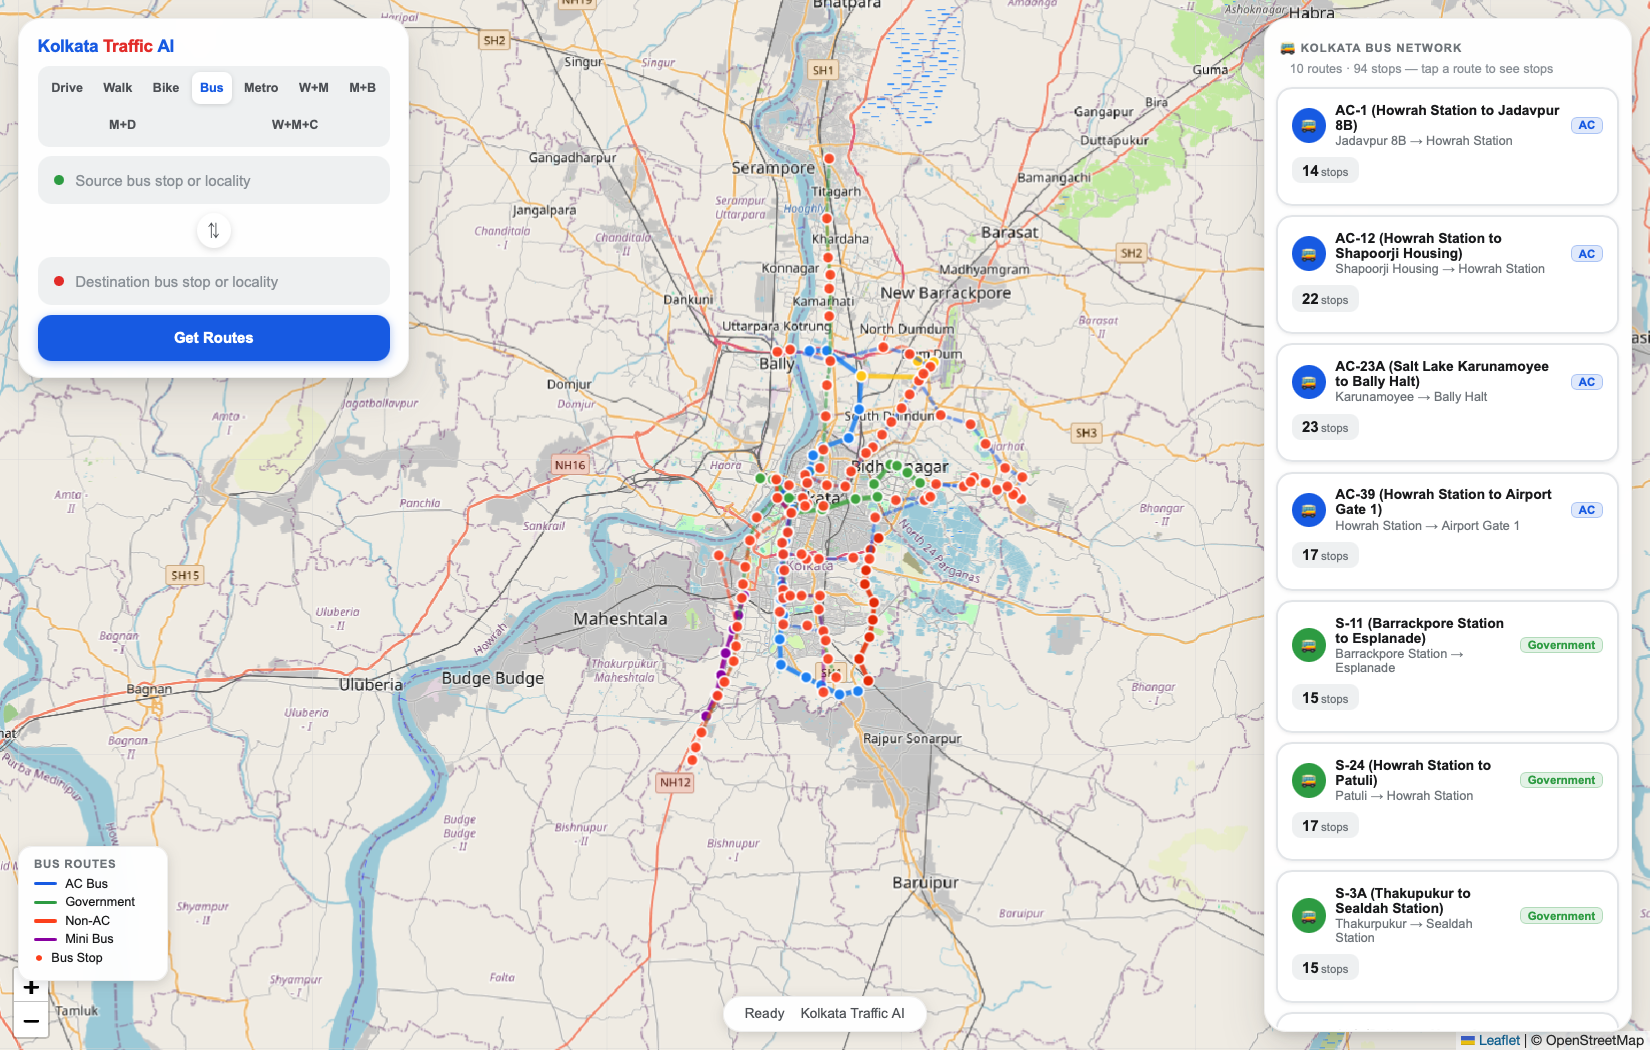
\includegraphics[width=1\linewidth]{bus.png}
\caption{Bus transit overlay and routing result.}
\label{fig:bus}
\end{figure}

% -------  Figure 4.5  -------
\begin{figure}[H]
\centering
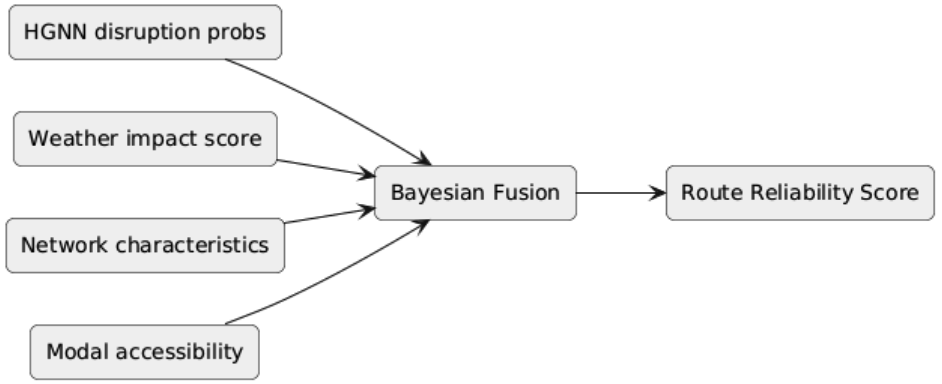
\includegraphics[width=\linewidth]{hgnn.png}
\caption{HGNN attention-based route explanation panel.}
\label{fig:explain}
\end{figure}

% -------------------------------------------------------------------
\section{Research Poster}
% -------------------------------------------------------------------

\noindent
The poster below was submitted as part of the GRISHMA programme deliverables.
It summarises the system architecture, methodology, and key findings.

\newpage
\thispagestyle{empty}
% Replace poster.pdf with your actual file when ready:
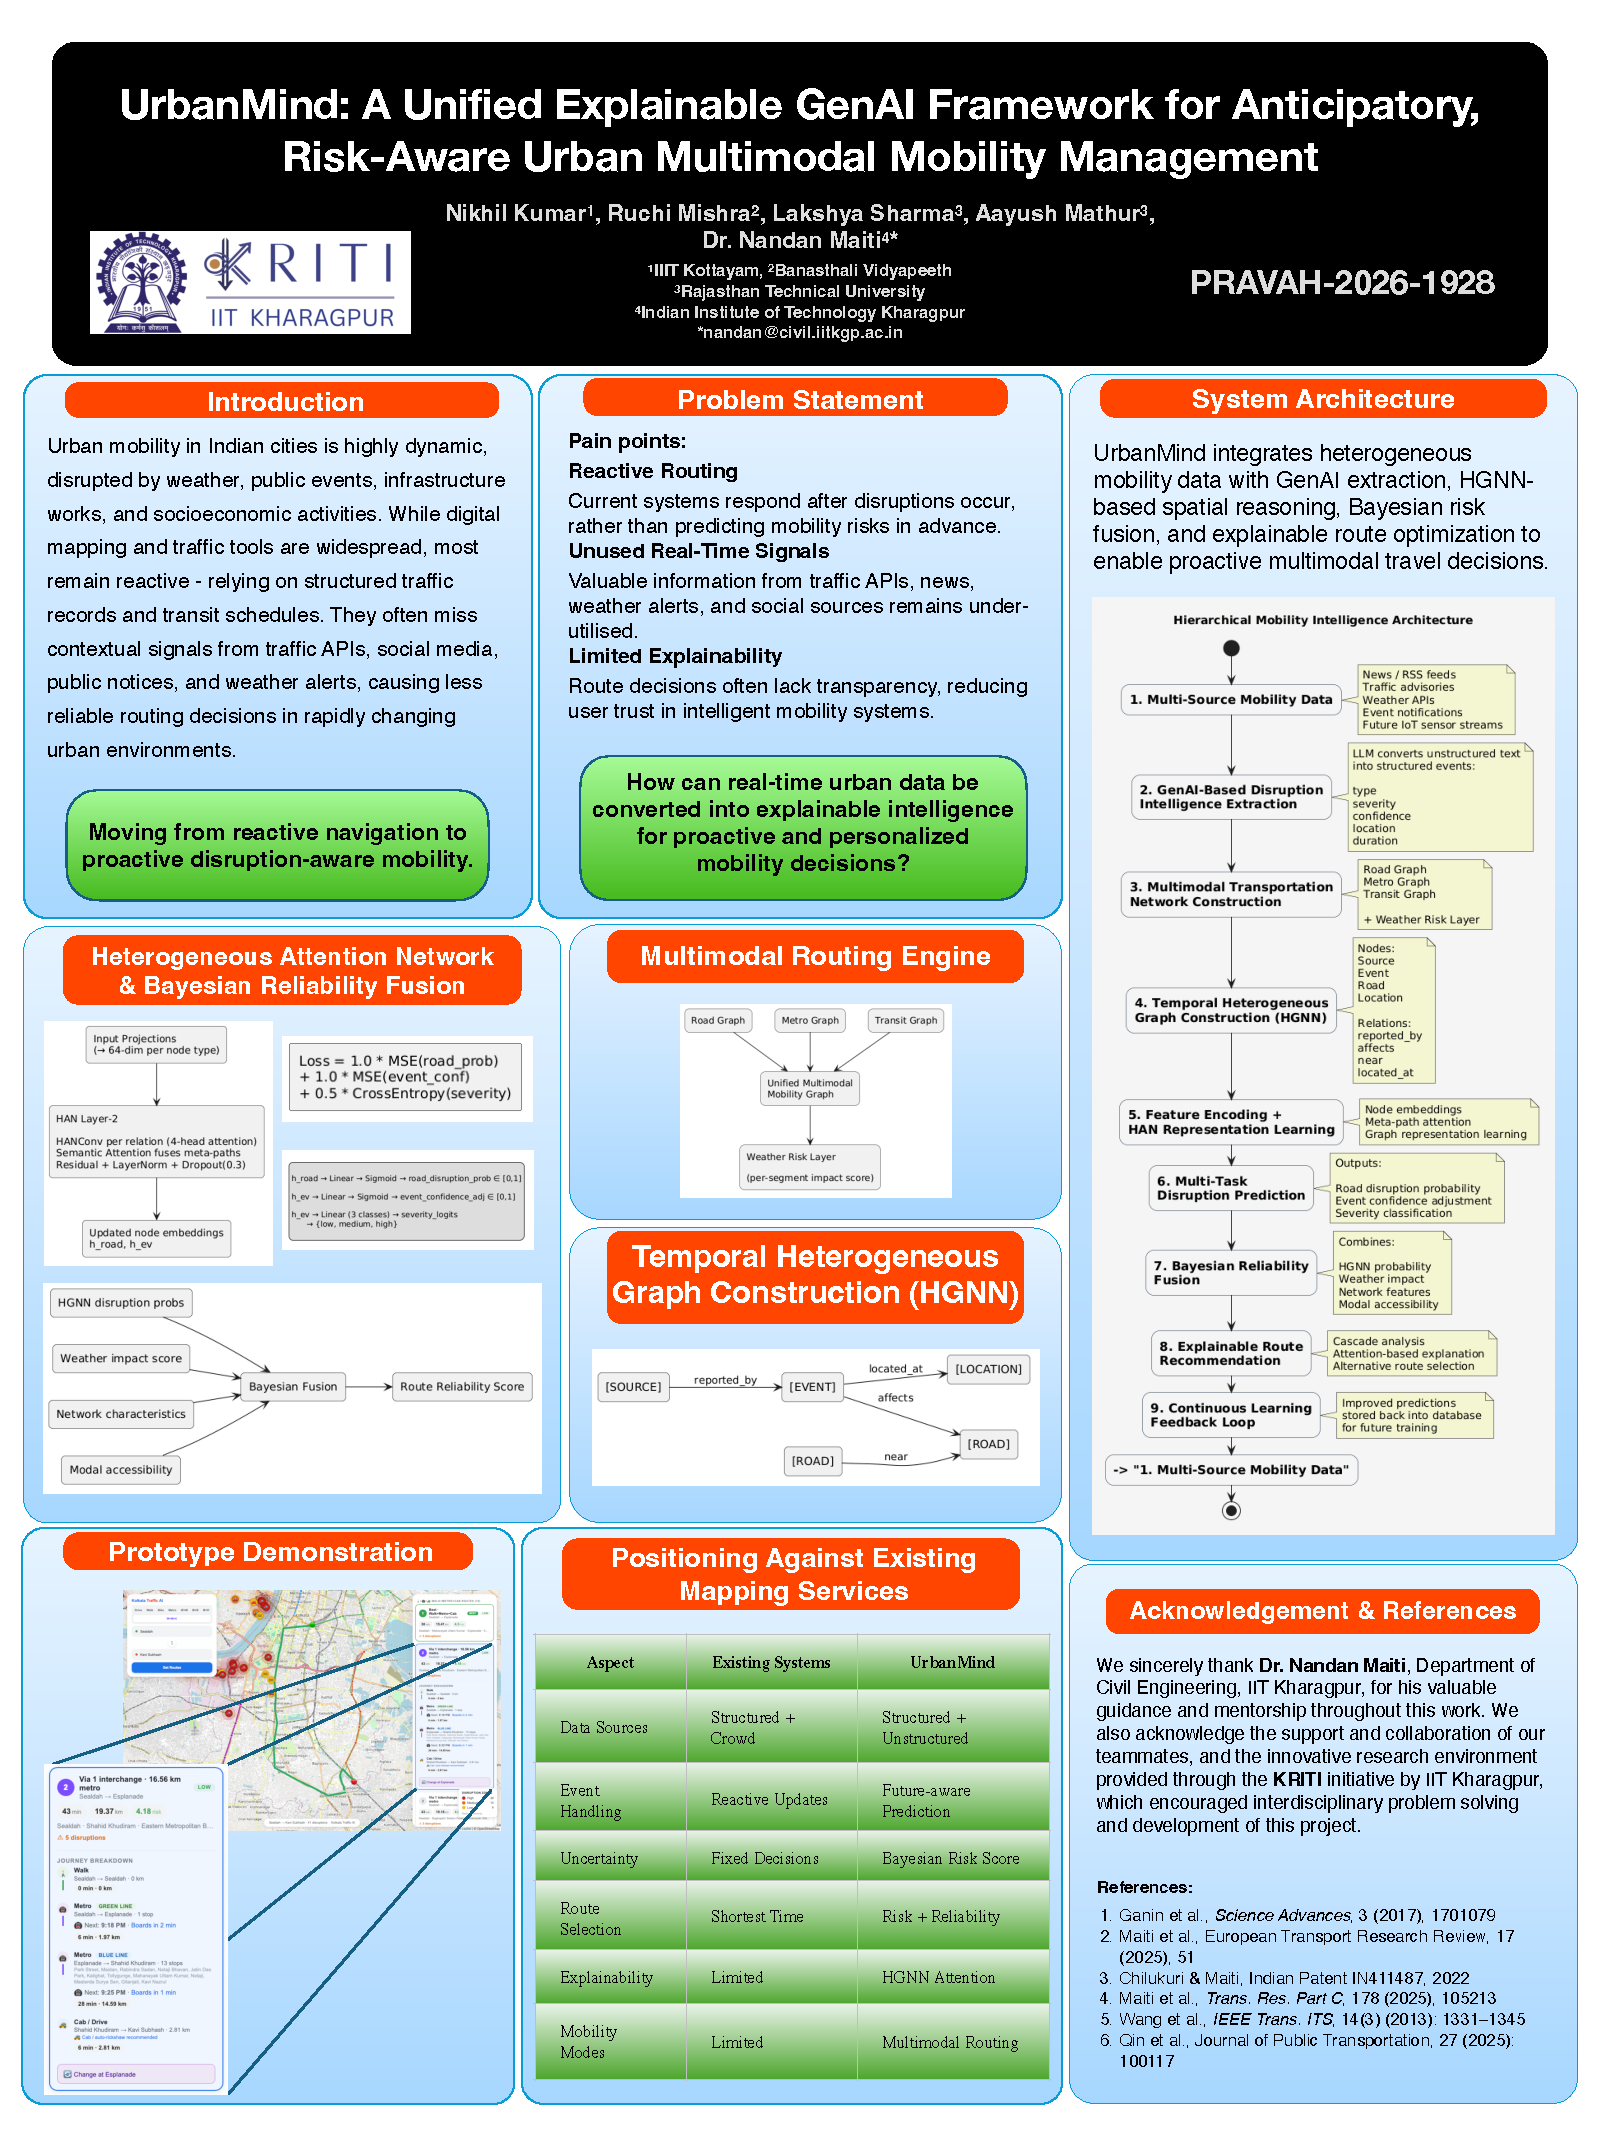
\includepdf[pages=1,scale=0.95]{Poster.pdf}
\newpage

\chapter{Conclusion and Future Work}

\section{Summary of Contributions}

\begin{table}[H]
\centering
\resizebox{0.7\textwidth}{!}{
\begin{tabular}{p{6cm}p{7cm}}
\toprule
\textbf{Contribution} & \textbf{Outcome} \\
\midrule
LLM extraction pipeline
  & Structured disruption events from 9 live sources;
    13 event types; mandatory location enforcement \\[4pt]
Temporal HGNN
  & City-wide confidence refinement; 3-output-head model;
    cascade road detection; attention-based explainability \\[4pt]
Bayesian probabilistic fusion
  & Per-road posterior disruption probabilities;
    time-of-day calibrated priors; HGNN blend \\[4pt]
Multimodal routing
  & 8 transport modes; full 5-line Kolkata Metro;
    BFS bus routing; OSMnx road/walk/bike graphs \\[4pt]
Weather risk assessment
  & Route-point sampling; Weather Severity Index (WSI)
    per candidate route \\[4pt]
FastAPI backend
  & 11 production endpoints; two-step design;
    2~s initial render regardless of LLM latency \\[4pt]
Frontend
  & Leaflet.js map; risk-coloured route lines;
    event markers; metro + bus overlays \\[4pt]
Database
  & Auto-migrating SQLite schema; HGNN feedback loop;\\
\bottomrule
\end{tabular}
}
\caption{Contributions made during the internship}
\end{table}

\section{Research Hypotheses -- Status}

\begin{table}[H]
\centering
\resizebox{0.7\textwidth}{!}{
\begin{tabular}{cp{7cm}p{4.5cm}}
\toprule
\textbf{ID} & \textbf{Hypothesis} & \textbf{Status} \\
\midrule
H1 & LLM signals improve disruption detection accuracy
   & Demonstrated qualitatively; ground-truth eval pending \\[4pt]
H2 & Risk-aware routing improves travel-time reliability
   & Layer~2 complete; Layer~3 (CVaR) in progress \\[4pt]
H3 & Explainable outputs enhance user trust
   & HGNN attention exposed via API; user study pending \\
\bottomrule
\end{tabular}
}
\caption{Hypothesis status at end of internship}
\end{table}

\section{Skills Acquired}

\begin{table}[H]
\centering
\begin{tabular}{ll}
\toprule
\textbf{Area} & \textbf{Specifics} \\
\midrule
LLM application dev    & LangChain LCEL, prompt engineering, JSON repair,
                         structured output \\
Graph neural networks  & Heterogeneous graph construction, HAN layers,
                         multi-task training (MSE + CrossEntropy) \\
Probabilistic ML       & Bayesian inference, likelihood ratios,
                         time-varying priors \\
Geospatial engineering & OSMnx, OpenStreetMap, GeoJSON, Leaflet.js,
                         Nominatim geocoding \\
Backend development    & FastAPI, Pydantic, SQLAlchemy, REST API design \\
Data engineering       & Multi-source ingestion, RSS/web scraping,
                         API rate-limit handling \\
\bottomrule
\end{tabular}
\caption{Technical skills developed}
\end{table}

\section{Future Work}

\begin{table}[H]
\centering
\resizebox{0.7\textwidth}{!}{
\begin{tabular}{cp{5.5cm}p{6cm}}
\toprule
\textbf{\#} & \textbf{Task} & \textbf{Details} \\
\midrule
1 & Layer 3 --- CVaR routing
  & Generalised edge cost combining travel time, risk, CO$_2$,
    and transfer penalty; CVaR optimisation for route selection \\[4pt]
2 & HGNN ground-truth training
  & Collect verified disruption labels from Kolkata Traffic Police;
    retrain severity and confidence heads on real data \\[4pt]
3 & GTFS-RT integration
  & Replace static metro/bus timetables with live GTFS-Realtime feeds \\[4pt]
4 & Natural language explanations
  & Layer~3 generates a plain-English justification per route
    recommendation (H3 full validation) \\[4pt]
5 & User trust study
  & Formal user experiment to validate H3 with Kolkata commuters \\[4pt]
6 & Multi-city deployment
  & Replace Kolkata OSM graph and transport datasets with those
    of another Indian metro for portability test \\
\bottomrule
\end{tabular}
}
\caption{Planned extensions}
\end{table}


\nocite{*}
\bibliographystyle{unsrt}
\bibliography{reference}

\end{document}
